\section{Exploring the Data}
\label{sec:Exploring the Data}

The data consists of two datasets: a relationships dataset describing relations between terrorists, and a terror attacks dataset documenting terror events by location and organisation.

%\subsection{Relationships Dataset}
%\label{subsec:Relationships Dataset}

\begin{figure}[H]
\begin{center}

        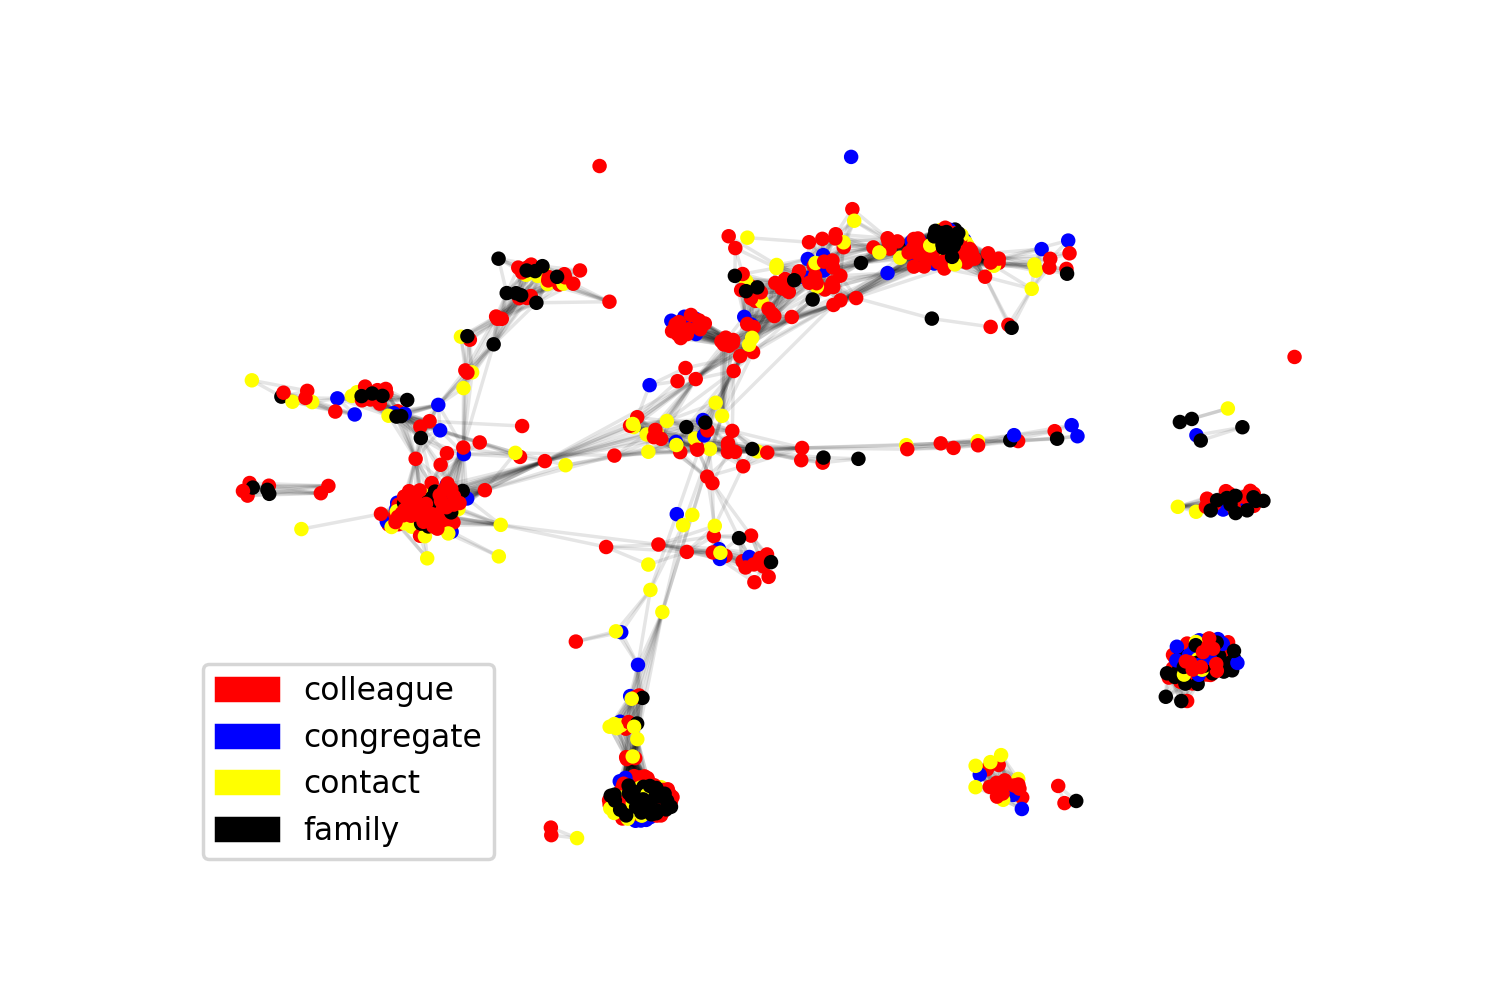
\includegraphics[width=.7\textwidth]{graphRel.png}
        \label{fig:graphLoc}
        \caption{Relationships dataset graph. The colouring of each node is related to its type of relation.}
        
\end{center}
\end{figure}

The relationships dataset represents the line graph of a network of relationships between terrorists. Each node represents a relationship between two terrorists. Two nodes are connected if they share a common terrorist. % and each edge a terrorist common to both connections. 
The label of each node relates to the nature of the relation between the two terrorists. It is an element of \{family, congregate, colleague, contact\}.

%\subsection{Terror Attacks Dataset}
%\label{subsec:Terror Attacks Dataset}

The terror attacks graph is built by connecting two nodes (terror attacks) if they share a common location. An other graph can be built by also connecting two terror attacks if they are perpetrated by the same organisation. This graph is not studied here.

\begin{figure}[t]
\begin{center}
    \begin{subfigure}[b]{0.45\textwidth}
        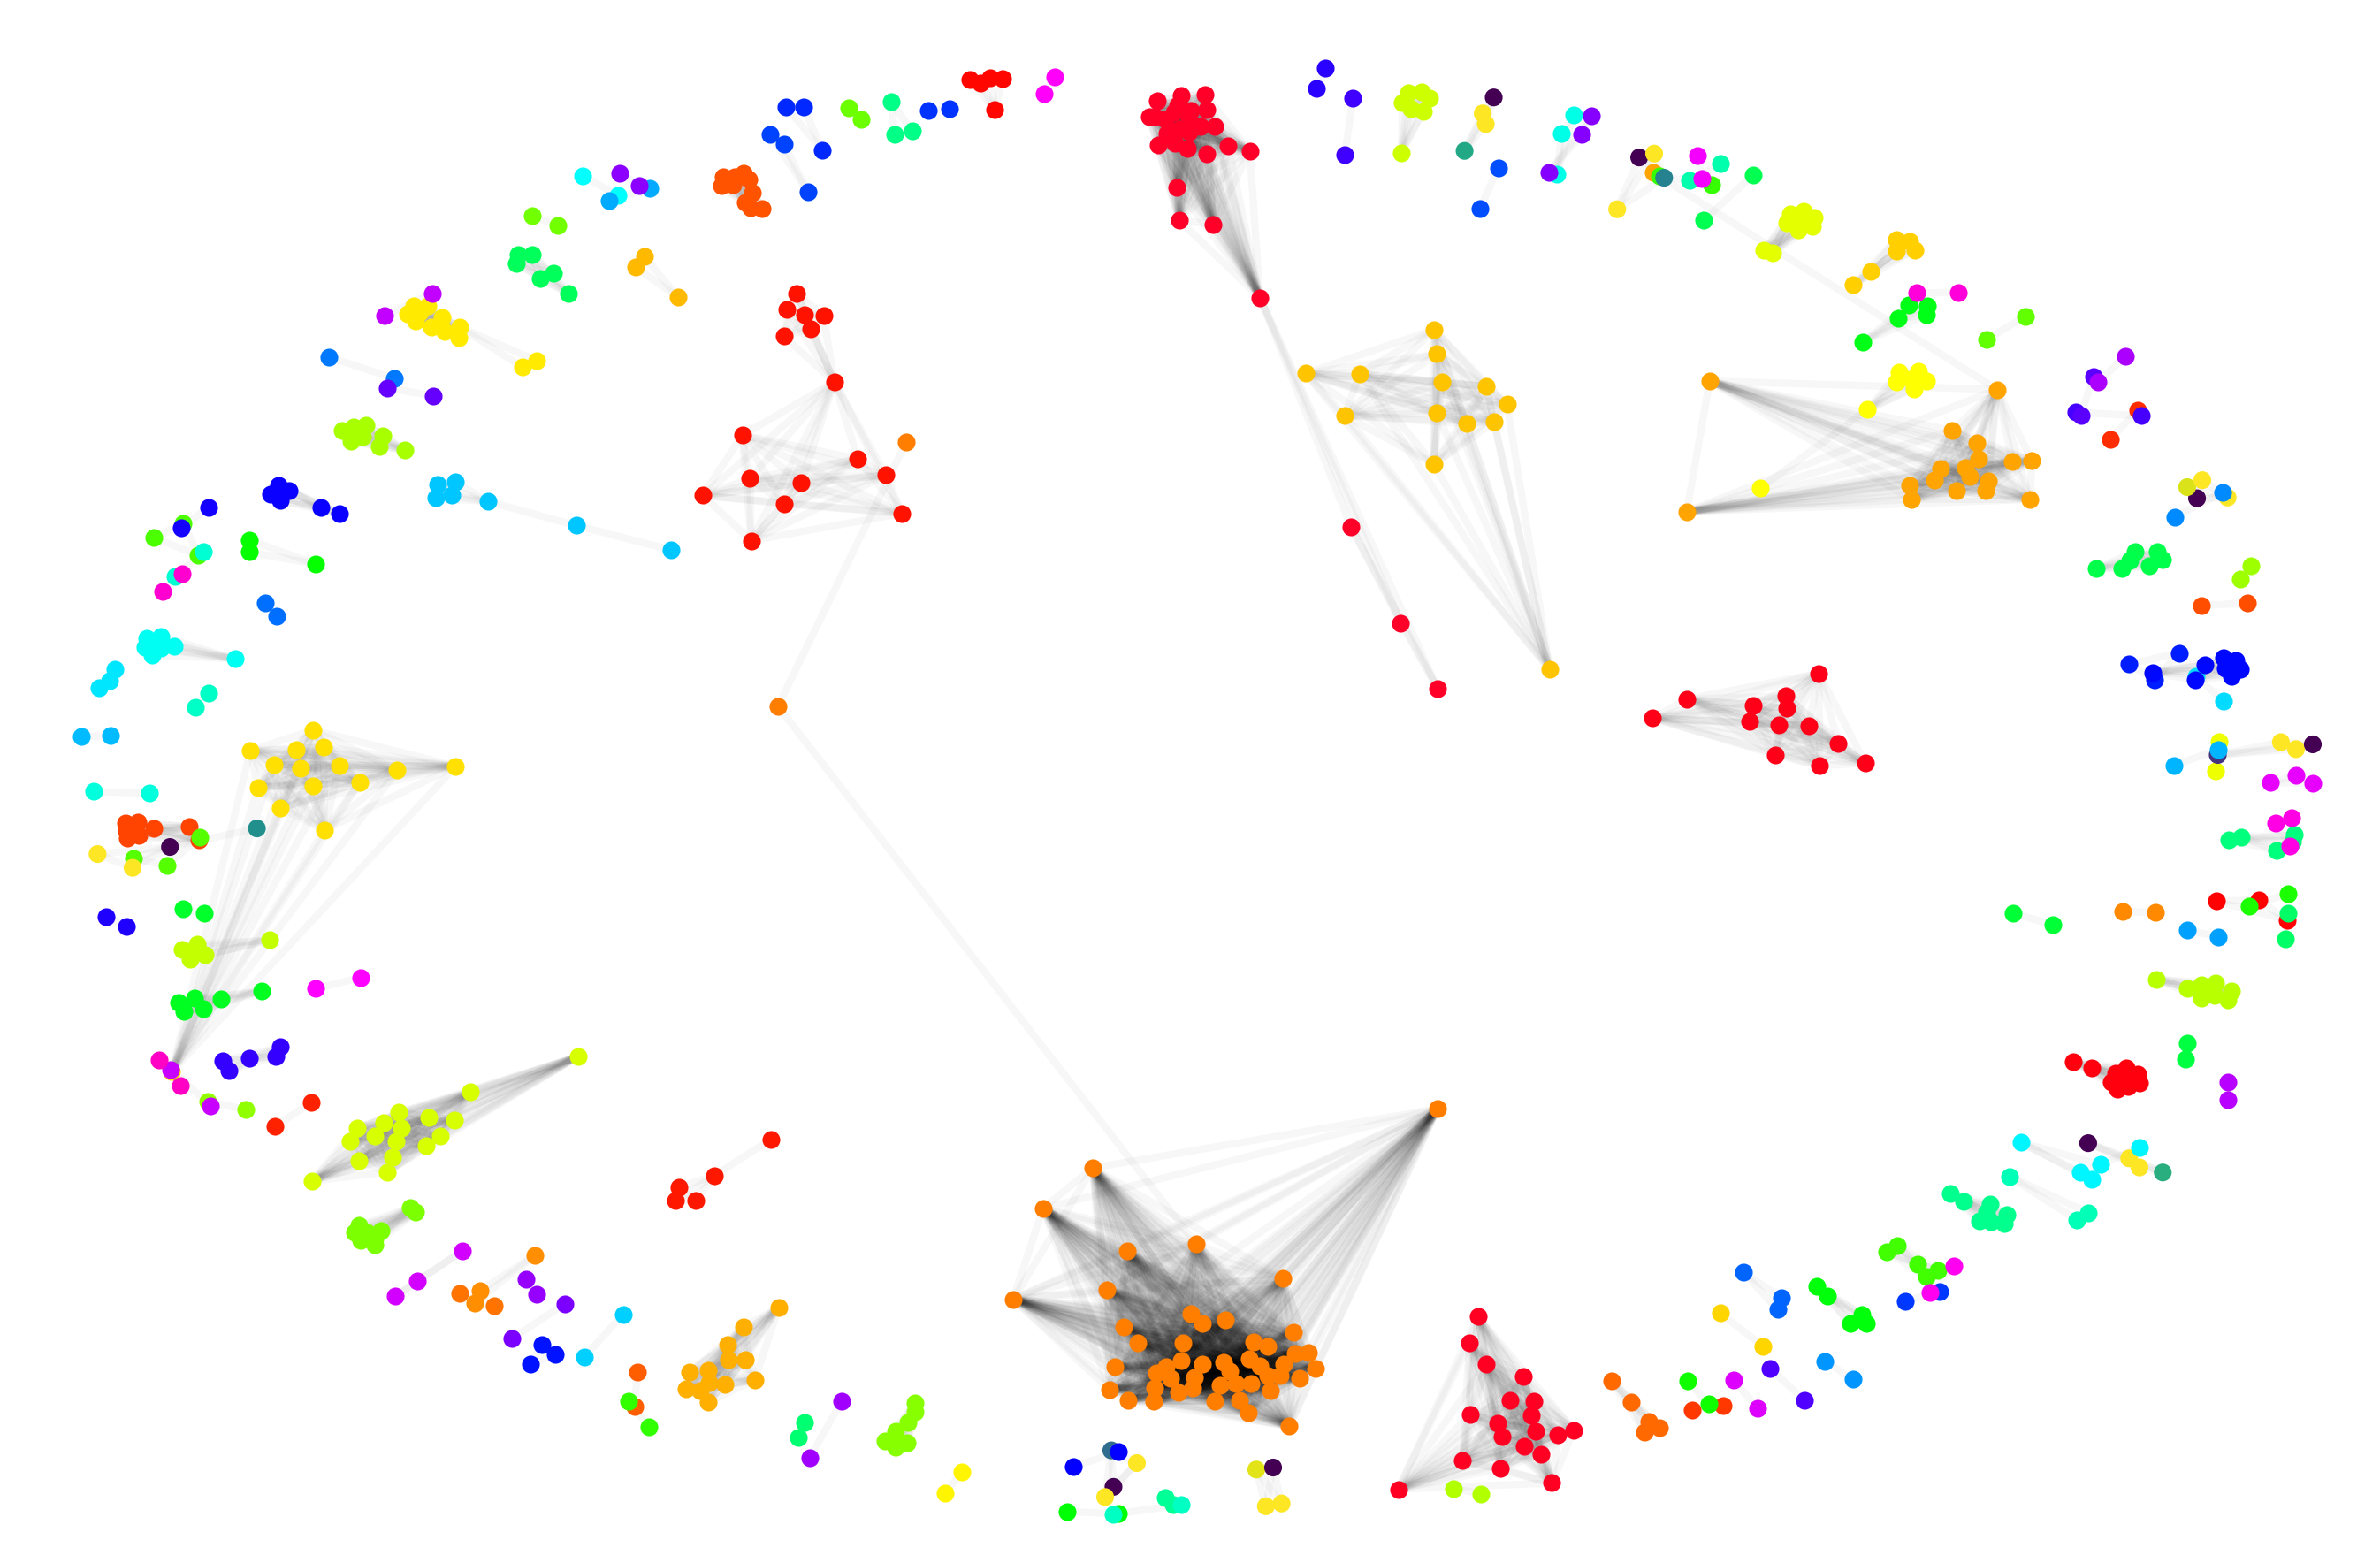
\includegraphics[width=\textwidth]{graphLoc.png}
        \caption{Terror attacks location graph, colouring by component ID}
        \label{fig:graphLoc}
    \end{subfigure}
    ~
    \begin{subfigure}[b]{0.45\textwidth}
        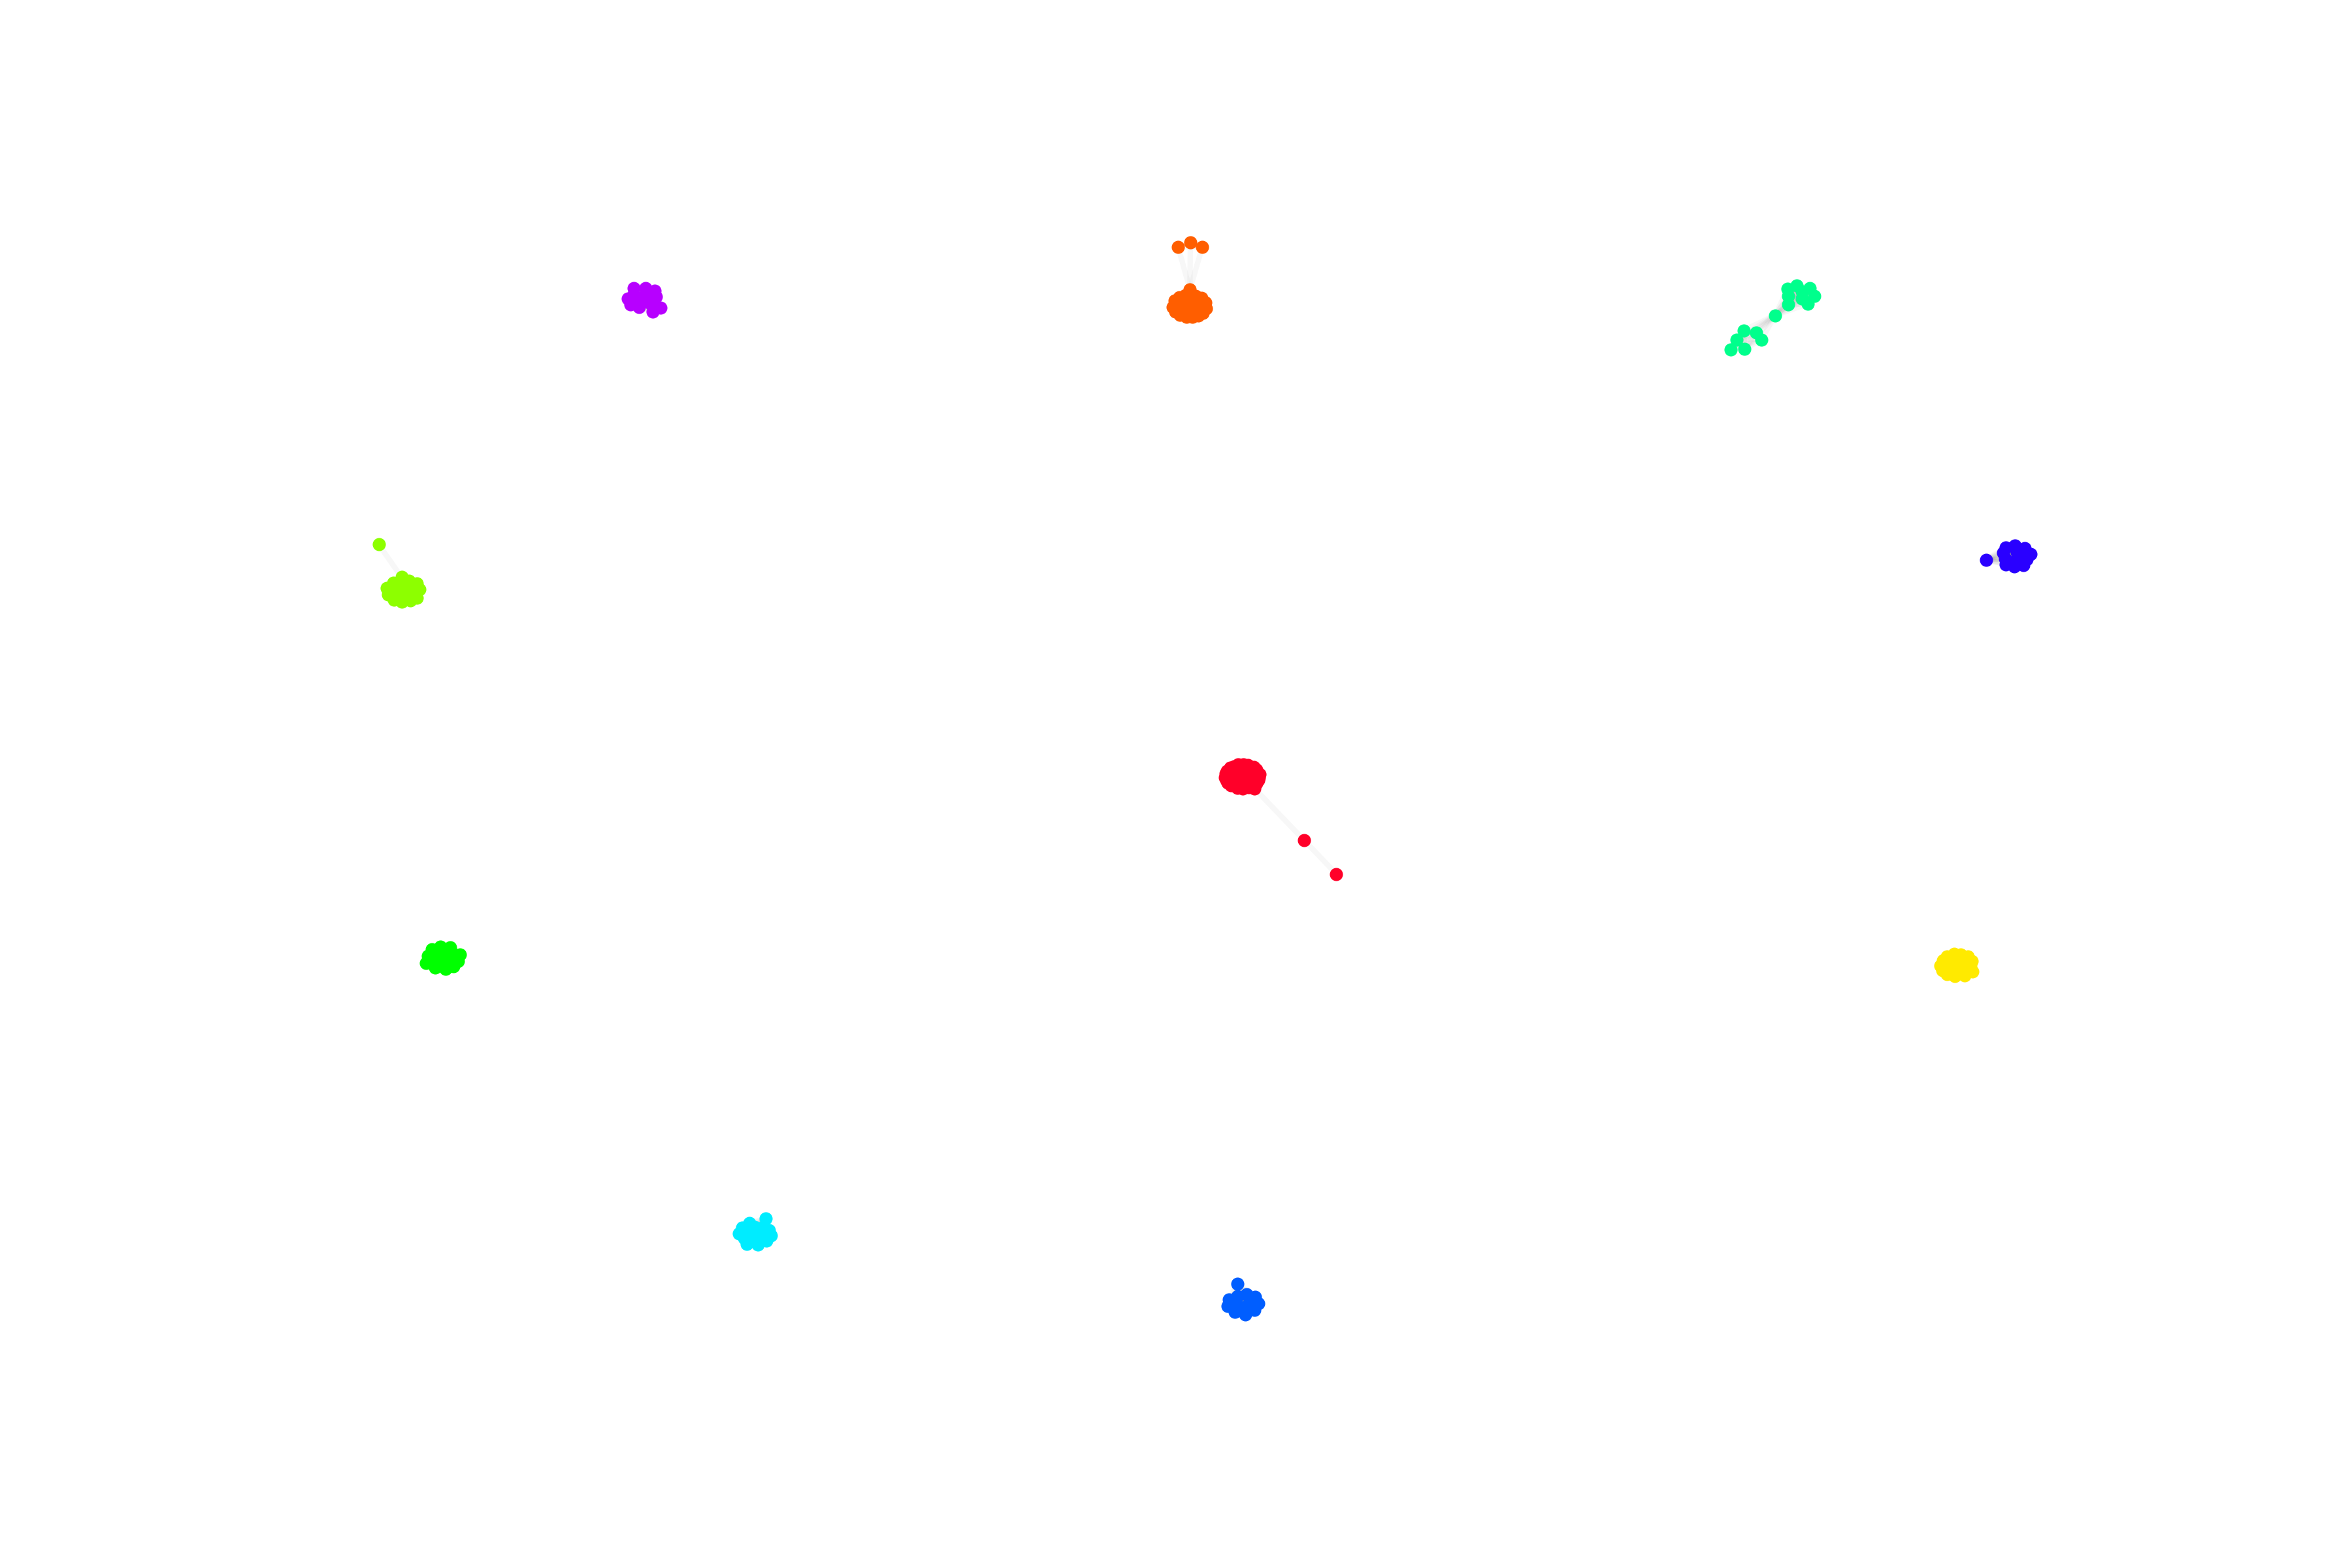
\includegraphics[width=\textwidth]{subGraph.png}
        \caption{Ten biggest components from the terror attacks location graph}
        \label{fig:subGraph}
    \end{subfigure}
\caption{Graphs from the terror attacks dataset}
\label{fig:graphPlots}
\end{center}
\end{figure}

Multiple issues have been found in this dataset:

\paragraph{Broadness} 
The dataset comprises attacks ranging from 1969 to 2005 and spanning the entire globe. Simple and relevant explanations for the graph formation or properties are not likely to be found, since the mechanisms behind two different attacks can be entirely different.

\paragraph{Structure} 
\label{par:Structure}
Half of the nodes are isolated, hence the topological information they carry in the graph is very limited. What is more, the construction of the graph implies a transitive relation inside connected components. Indeed, let $a$, $b$ and $c$ be terror attacks from the same connected component. Let ``$a\sim b$'' mean that terror attacks $a$ and $b$ took place close to each other. Then
\begin{equation}
\text{If } \left ( a \sim b \text{ and } b \sim c \right )  \text{ then probably } a \sim c
\label{eq:transitivity}
\end{equation}
This property translates into connected component that are almost complete -- hence bearing little topological information.

\paragraph{Reliability} 
As expected, errors have been found in the data. For example nodes
 \texttt{Djibouti\_Youth\_Movement\_19900927} 
 and 
 \texttt{Armed\_Islamic\_Group\_19950711} 
 have been connected, whereas the first attack took place in Djibouti~\cite{amnesty1991} and the second one in Paris~\cite{nouvelObs2007}. Hence algorithms using the data must tolerate some error in order to avoid overfitting.

\paragraph{Incompleteness}
The dataset has been constructed from publicly available sources~\cite{ZSG2006}. Because of the sensitivity of the data behind terrorist attacks and relationships, some of it is classified, making the dataset incomplete.

Further properties of the graphs are discussed below.

%Similarly to relationships datasets, we have found that the terrorist attacks dataset have very highly connected components, implying transitivity. 
%If attack $a$ took place close to $b$, and attack $b$ took place close to $c$, then it is probable that attack $a$ took place close to $c$.

